\section{Resultados}

Para a demodulação do sinal FM, foi obtido o seguinte gráfico:

\begin{figure}[!h]
    \centering
    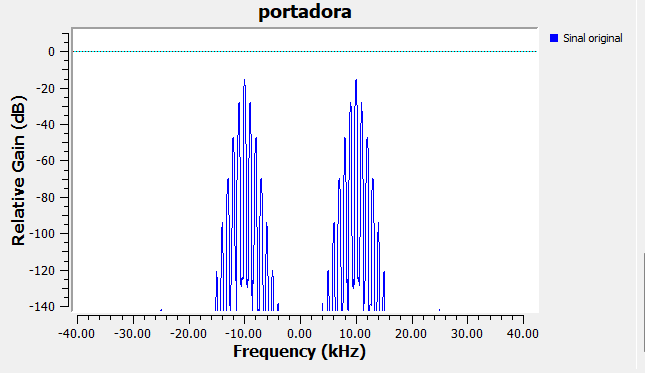
\includegraphics[width=0.5\textwidth]{images/sinal_fm_p.png}
    \caption{Gráfico do sinal demodulado.}
    \label{fig:resultado_demodulacao}
\end{figure}

aumentado a amplitude do sinal mensagem, tempo mais armonicas sendo geras.

Na demodulação do sinal FM, foi observado que o aumento da amplitude do sinal mensagem resultou em um maior número de harmônicas sendo geradas. Isso é esperado, pois a modulação em frequência (FM) é sensível à amplitude do sinal de mensagem, e um aumento na amplitude leva a uma maior variação na frequência da portadora, resultando em uma maior complexidade espectral do sinal demodulado.

\begin{figure}[!h]
    \centering
    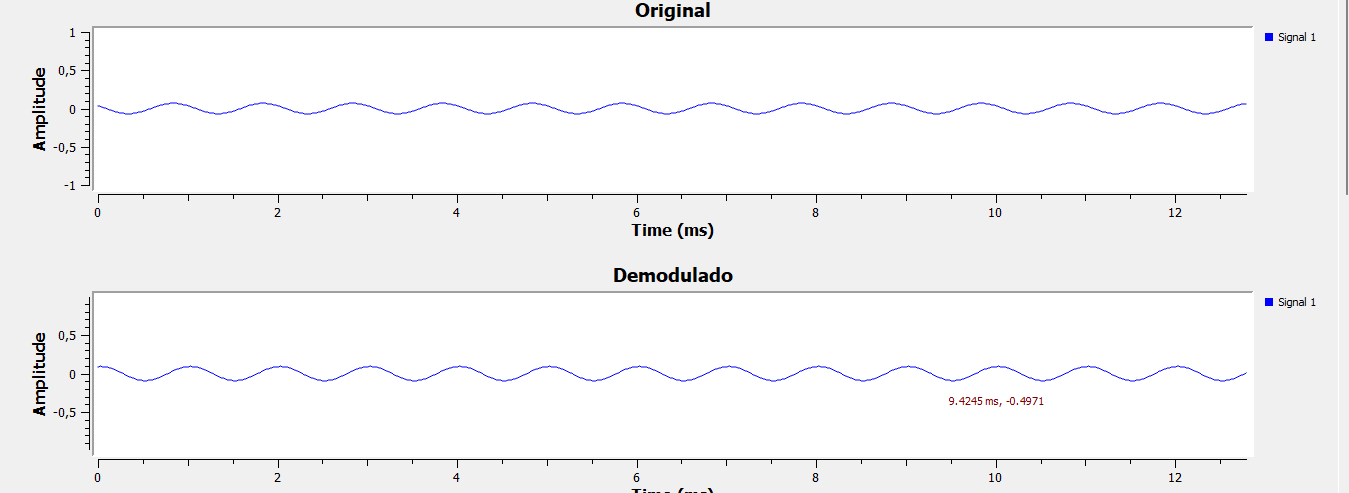
\includegraphics[width=0.5\textwidth]{images/cdm.png}
    \caption{Gráfico do sinal demodulado.}
    \label{fig:resultado_demodulacao}

\end{figure}

